\documentclass[../main.tex]{subfiles}

\begin{document}

\chapter{Introduction}\label{cha:introduction}
\minitoc

\section{Context}
  \todo{Nowadays problems (large-scale \ldots) need to decompose, problems with security Stuxnet \cite{Langner2011} and other attacks (use examples in~\cite{DingEtAl2018})}%
  \todo{ more examples in \cite{Bindra2017}}

\section{Motivation and Contributions}
Due to the increased computation capabilities of computers in recent years,
now we can solve some problems which were then not solvable in reasonable time.
Thus the \emph{renaissance} of some optimization based methods, such as \todo{Neural networks} and \todo{Artificial Intelligence}.
For other more common methods such \mpc~\cite{GarciaEtAl1989}, this development meant solving bigger problems in less time, sometimes even in realtime~\todo[add realtime MPC]{\cite{BesselmannEtAl2008}} and using small computation units that can fit in the palm of a hand~\cite{BanguraMahony2014}.
But still, for some large scale systems, the calculation need to be distributed into many computation units.

This work studies what happens when these computation units do not work collaboratively.
And for a specific decomposition we search for a method to mitigate the effects of this non-cooperative behavior.

To give a general view to the reader and to serve as a main take-out of the possible effects, we give a simple qualitatively example, which will be retaken quantitatively in another section of this work.

\begin{example}[Effects of a malicious agent]
  Imagine we have a system where we want to minimize an overall objective.
  For this a number of agents interact.
  In the decomposition used in this work the agents need to exchange values with another agent which referees what we call a negotiation.
  The coordinator sends all agents a message, and each agent responds the coordinator by sending a message which depends on the original message. We can see a scheme of the exchanges in Fig.~\ref{fig:ex_exchange_agents}

  % \pagebreak

  % \begin{minipage}[t]{1.0\linewidth}
  %   \vspace{.25cm}
  % \end{minipage}
  \begin{figure}[H]
    \centering
    \begin{tikzpicture}[font=\small,thick,node distance=3*0.6180cm and 0.6180cm,every node/.style=rectangle,
      mpcSmall/.style={fill=mpc_agent, minimum height=0.6180*2cm, minimum width=2cm},
      coordinator/.style={fill=mpc_coordinator, minimum height=0.6180*3cm, minimum width=6cm},
      ]

      \node[draw, mpcSmall,] (block1) {\small Agent 1};
      \node[fill=none, draw=none, right=of block1,] (mult) {\bf $\dots$};
      \node[draw, mpcSmall, fill=mpc_agent, right=of mult,] (blockM) {\small Agent M};
      \node[draw, coordinator, below=of mult,] (coordinator) {Coordinator};

      \draw[-latex,line width=1pt,red] (block1.south)+(0.4,.0) -- ( coordinator.north -| {$(block1.south)+(0.4,.0)$}) node [right,midway] {\faUserSecret};
      \draw[latex-,line width=1pt] (block1.south)+(-0.4,0) -- (  coordinator.north -| {$(block1.south)+(-0.4,0)$});
      \draw[-latex,line width=1pt] (blockM.south)+(0.4,.0) -- ( coordinator.north -| {$(blockM.south)+(0.4,.0)$});
      \draw[latex-,line width=1pt] (blockM.south)+(-0.4,0) -- (  coordinator.north -| {$(blockM.south)+(-0.4,0)$});
    \end{tikzpicture}
    \caption{Exchange between agents.}\label{fig:ex_exchange_agents}
  \end{figure}

  Observe in Fig.~\ref{fig:ex_exchange_agents} that Agent 1 sends a modified version of the message it was supposed to send. This can be considered as an attack \todo{called \fdi, as we will see later}.

  In Fig.~\ref{fig:change_in_j}, we can see the effects on the overall objective $J^{\star}$ (in blue) when agent 1 changes a different version of the original message.
  \begin{figure}[H]
    \centering
    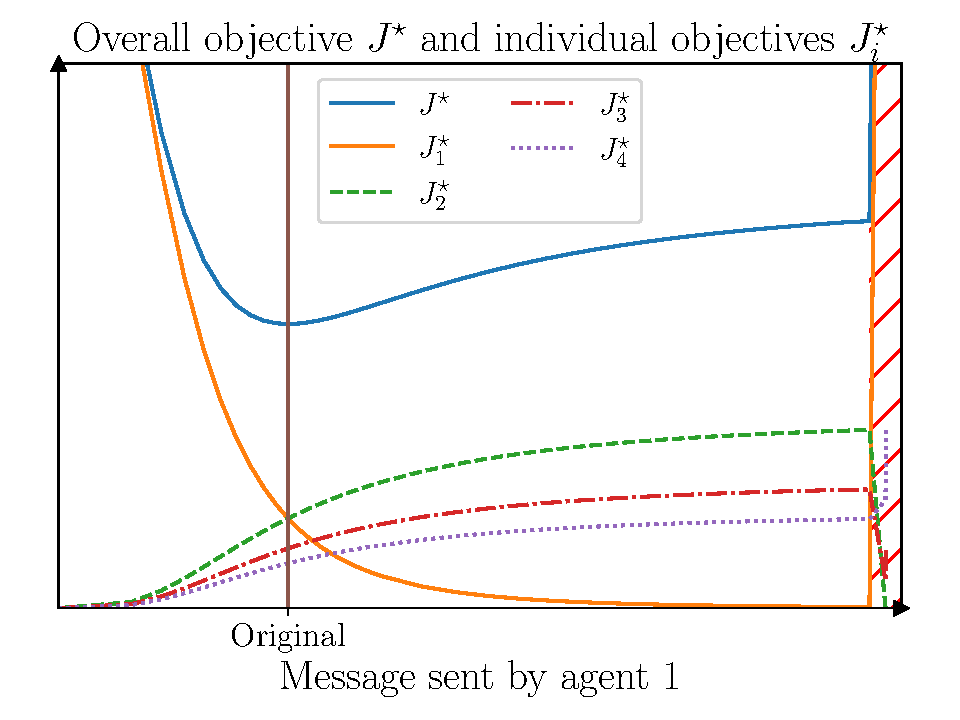
\includegraphics[width=.55\textwidth]{../img/qualitative_example.pdf}
% ./docstheseplot -o ../../docs/img/quantiteAvecTriche4 -i  ../../data/matlab/tricheQuantite/dmpcQuantity4systemsTriche_.mat --quantiteAvecTriche4
    \caption{Change in objectives depending on message sent by agent 1.}\label{fig:change_in_j}
  \end{figure}
  Observe that the blue curve has its minimum value only when the message is the original one, every other message makes the resulting system sub-optimal.

  The red hatched area represents a set of messages that agent 1 can send that destabilize the system.
\end{example}

From the simple example we can se the two main effects: Loss of optimality and eventual \todo{total breakdown}.

In this work we look forward to answer the following questions for a specific case which will be formally presented in the next section:

\simplebox{
  \begin{itemize} \bfseries
    \item Can we detect an attack?
    \item Can we identify the ill-intentioned agent(s)?
    \item Can we mitigate the effects of the attack?
  \end{itemize}
}

To answer this questions, we divide this work into two parts.

In the first part



Section to position this work before others

Since those questions are still open, this work has as objective to discuss these questions by analyzing the recent literature and schematizing the security in decomposition methods for Model Predictive Control passing by the following items:
\begin{itemize}[label=$\bullet$]
  \item decomposition methods;
  \item topology;
  \item points of vulnerability;
  \item how malicious agents can benefit from such vulnerabilities;
  \item effects on the overall system;
  \item possible ways to mitigate.
\end{itemize}
We use some conclusions of the discussion to develop safe algorithms for a \dmpc\ framework.

\section{Publications}
The work and discussion presented in this thesis yielded the following publications
\begin{itemize}
  \item Published
        \begin{description}
          \item[\cite{NogueiraEtAl2021}] Conference article for the SysTol'21
        \end{description}
  \item Under Review
  \item In Preparation
\end{itemize}



% \chapterEndOrnament
\printbibliography
\end{document}
